\chapter{MEASUREMENTS OF THE VISCOSITY OF THE QUASI-LIQUID LAYER AT THE SURFACE OF ICE-I$_\mathrm{h}$}\label{chap:QLL}

\begin{flushright}
\textit{''Why do snowflakes always fall as flat structures with six corners?''} \\
-Joannes Kepler (1611) \\
\end{flushright}

In the hydrodynamic friction regeime for a slider passing over an ice surface, three distinct forces contribute to the overall observed friction; the solid-liquid friction between the ice and quasi-liquid layer (QLL), the viscous shearing of the qll, and the solid-liquid friction between the qll and the slider. In Chapter \ref{chap:Friction}, we presented facet-dependent friction coefficients for the basal, prismatic, 14\degree~pyramidal, and secondary prism ice-I$_\mathrm{h}$ / water interfaces. In this chapter, we discuss the contribution of the viscous shearing of the qll at the basal and prismatic ice-I$_\mathrm{h}$ / vapor interface.



\section{Computational Methods}
TIP4P-Ice basal and prismatic ice-I$_\mathrm{h}$ primitive crystals were constructed following the procedure described in Chapter \ref{chap:Methods}. These primitive cells were then reoriented so that the desired crystal face was exposed to the $y$ axis, then replicated in the $x$ and $z$ dimensions to form large sheets. The sheets were then replicated in $y$ until the basal crystal was 12 bilayers thick, and the prismatic cyrstal was replicated to a width of approximately equal to the basal crystal. Dimensions and number of molecules in each system are found in Table \ref{tab:qll-method}.


\begin{table}[h]
\centering
\caption{SIZES OF THE VAPOR EXPOSED ICE-I$_\mathrm{h}$ / QUASI-LIQUID LAYER SIMULATIONS\label{tab:qll-method}}
\begin{tabular}{r|c|ccc}
\hline
\hline
 Interface & $N_\mathrm{ice}$ & $L_x$ & $L_y$ & $L_z$ \\
\hline
Basal  $\{0001\}$                           & 46,080 & 185.24 & 44.04 & 186.06 \\
Prismatic  $\{10\bar{1}0\}$            & 55,000 & 192.47 & 49.14 & 181.61\\
\hline
\hline
\end{tabular}
\begin{flushleft}
Box dimensions are given in \AA.
\end{flushleft}
\end{table}


The $y$-dimension of the simulation box was then set to 300~\AA~ to allow for a surface premelt to form, and each system was equilibrated to 265~K~. The resulting systems exposed two interfaces, one toward positive $y$ and the other towards negative $y$. The equilibration was conducted under a constant pressure and temperature integrator, allowing the $x$ and $z$-dimensions of the simulation cell to relax and alleviate any crystal strain. Following this the systems were then equilibrated under a constant volume and temperature integrator, and lastly under a constant volume and energy integrator. During these simulations, the width of the crystal (in the $y$-dimension) was monitored to ensure no appreciable crystal melt occurred.

Once equilibrated, a shear stress was applied only to molecules within the QLLs using the velocity shearing and scaling variant of reverse non-equilibrium molecular dynamics described in Chapter \ref{chap:Methods}.\cite{Kuang2012} The VSS-RNEMD exchange regions were defined to incorporate molecules from both the top and bottom interfaces, as seen in Figure \ref{fig:qll-rnemd}. Both the tangential density and tetrahedrality profiles were used to determine the $y$-width of the exchange VSS-RNEMD regions. In Chapter \ref{chap:Str}, we found the tetrahedrality at the Gibbs dividing surface for ice-I$_\mathrm{h}$ / water interfaces to be $q^{Gibbs} \sim$0.84. Here, we have used $q^{Gibbs}$ as the cutoff value between the QLL and the ice. All molecules with $q < q^{Gibbs}$ are denoted as QLL molecules, while those with $q > q^{Gibbs}$ are denoted to be ice. This cutoff coincides with a minimum in the tangential density profiles, as seen in the top and bottom panels of Figure \ref{fig:qll-rhoq}.


\section{Distance Dependence of Viscosity from the Ice Surface}
As seen in Figure \ref{fig:qll-rhoq}, the QLLs at the surface of the
basal and prismatic crystals form a bilayer. Following Neshyba
\textit{et al.}, we denote the following definitions; molecules within
the ice are labeled as $\mu_{i}$, where each $i$ denotes a unique
density peak in the ice, molecules in the QLL layer closer to the ice
are labeled as $\epsilon_{2}$, and molecules in the outter portion of
the QLL bilayer are labeled as $\epsilon_{1}$.\cite{Neshyba2009} Due
to their relative distances from the underlying crystal, molecules
within layers $\epsilon_{2}$ and $\epsilon_{1}$ experience vastly
different local environments. Water molecules within $\epsilon_{2}$
located closer to the ice experience significantly more drag than
those closer to the vapor. Therefore, we expect a noticeably different
sheaer viscosity for the molecules located in $\epsilon_{2}$ and
$\epsilon_{1}$. 

The shear viscosity, $\eta$, of the QLL can be determined using the linear
constitutive relation for a shear stress imposed across a liquid.
\begin{equation}\label{eq:qll-visco}
j_z(p_x) = \eta \frac{\partial v_x}{\partial z}
\end{equation}
Since the QLLs are composed of multiple layers of varying densities
and local structures, their response to the shear stress may vary. Due
to this, we have computed $\eta$ for thin slices of $y$ through the
QLLs as seen in Figure \ref{fig:qll-vx}.

\begin{figure}
\includegraphics[width=\linewidth]{Figures/qll-vx}
\caption{\label{fig:qll-vx} Shearing profiles of the basal QLLs for
  molecules close to the underlying ice surface ($\epsilon_{2}$) and
  molecules closer to the vapor ($\epsilon_{1}$). }
\end{figure}                


\begin{figure}
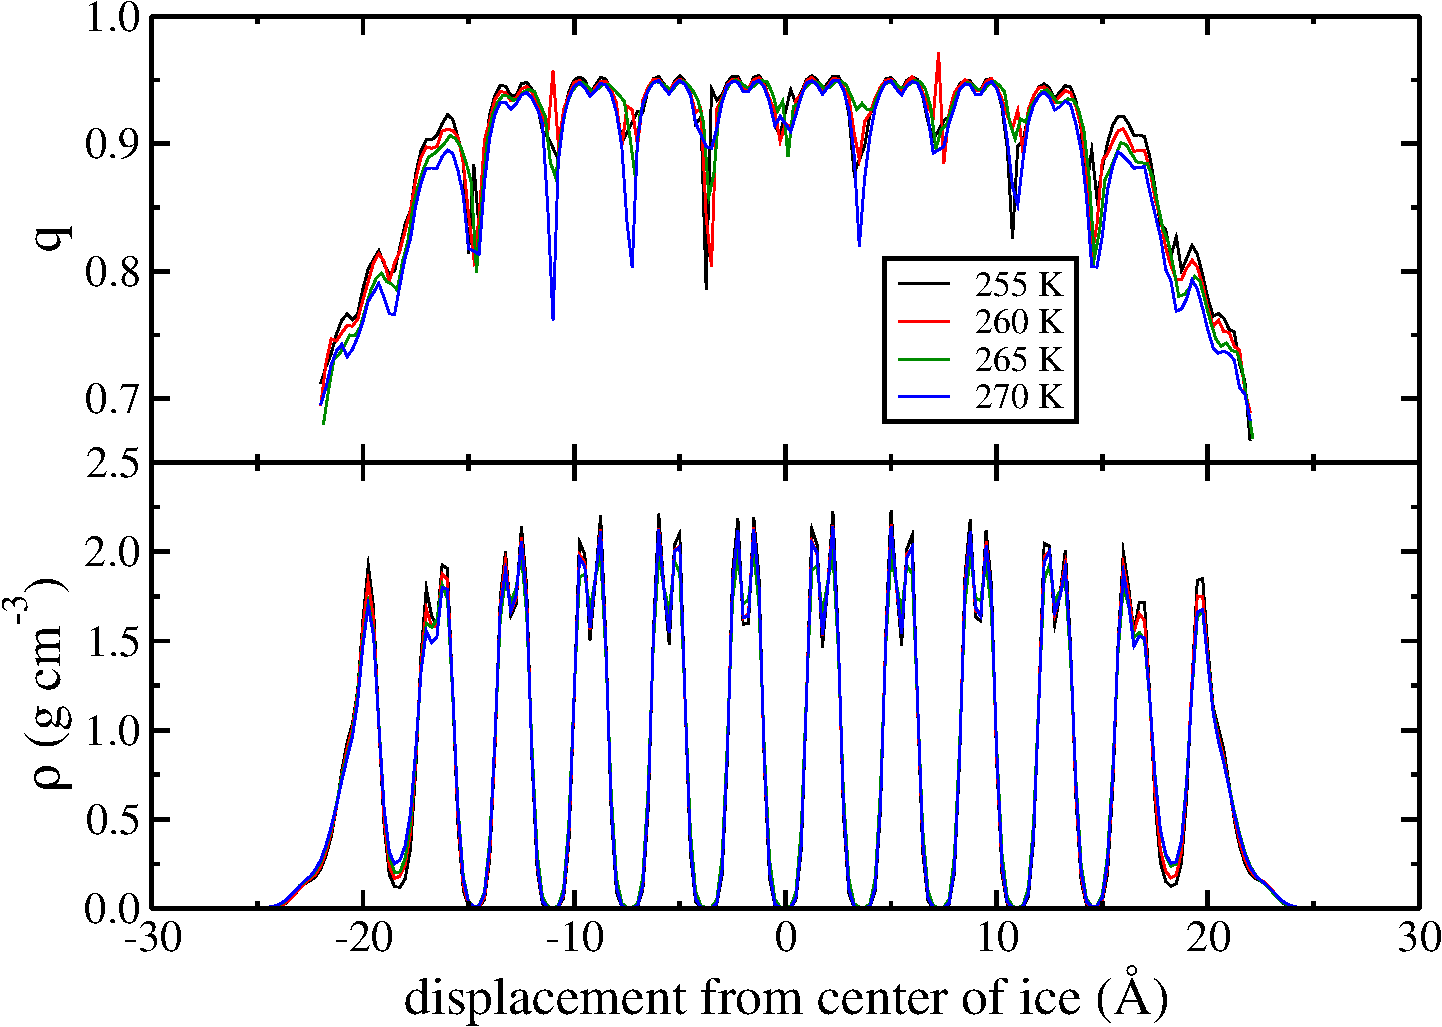
\includegraphics[width=\linewidth]{Figures/basal_rhoq}
\caption{\label{fig:basal_rhoq} Shearing profiles of the basal QLLs for
  molecules close to the underlying ice surface ($\epsilon_{2}$) and
  molecules closer to the vapor ($\epsilon_{1}$). }
\end{figure}                


\begin{figure}
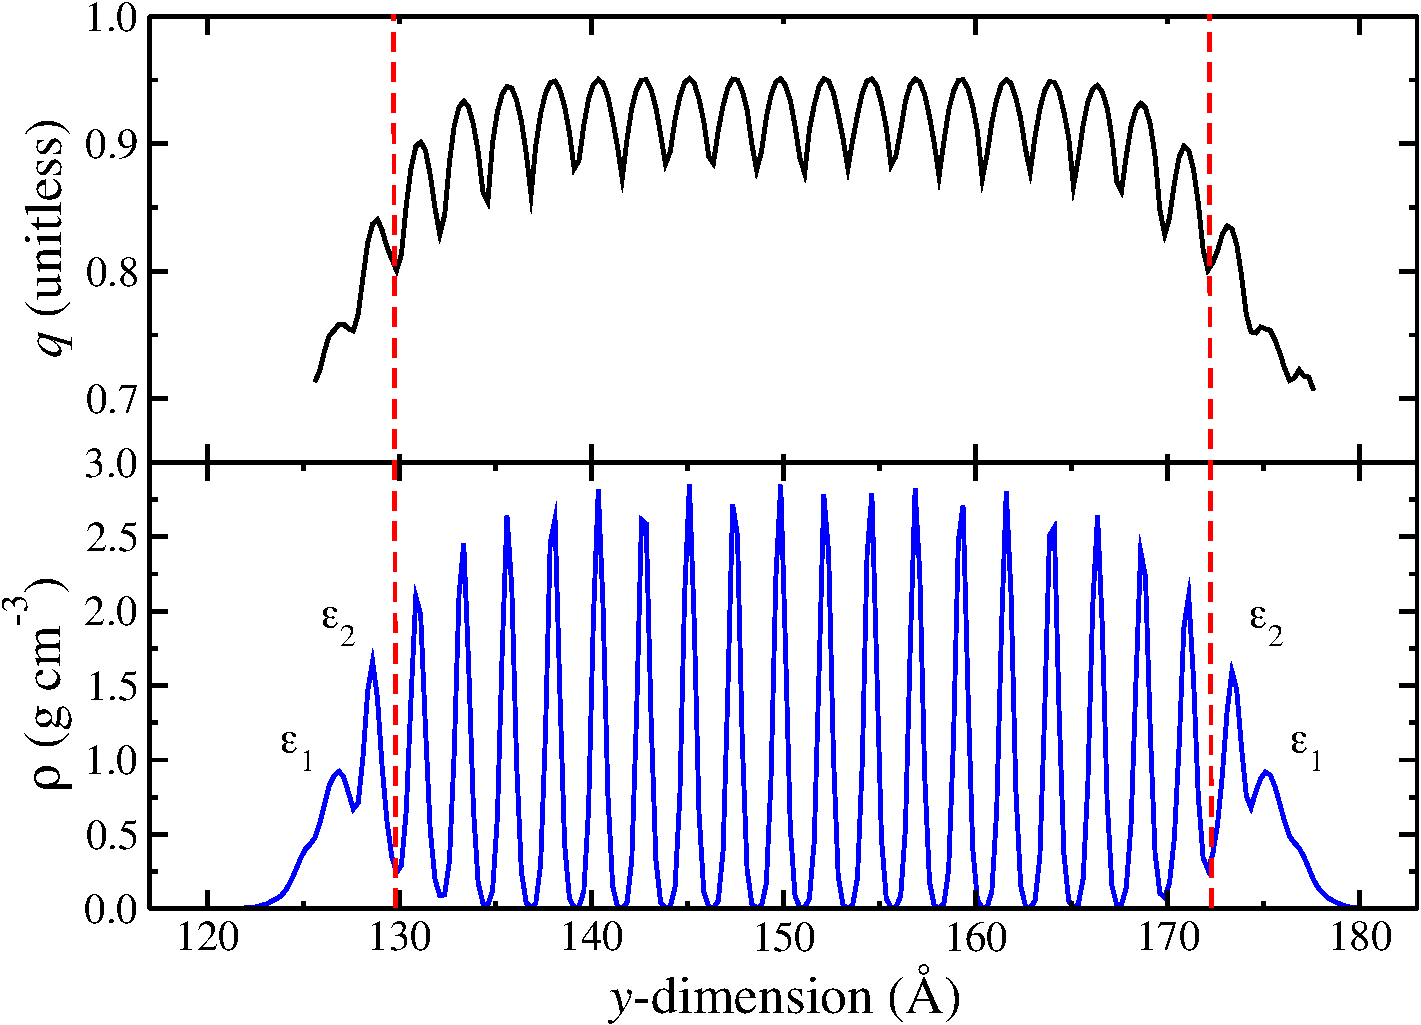
\includegraphics[width=\linewidth]{Figures/prism_rhoq}
\caption{\label{fig:prism_rhoq} Shearing profiles of the basal QLLs for
  molecules close to the underlying ice surface ($\epsilon_{2}$) and
  molecules closer to the vapor ($\epsilon_{1}$). }
\end{figure}                



Previous estimates of the viscosity of the quasi-liquid layer (QLL) on the surface of
ice have come from the Stoke's-Einstein relation, which relates the
diffusion of the surface molecules to the viscosity. However,
molecules at the surface of ice which are transitory in the vapor
phase can skew the results, as their mean-square displacements will be
much larger than those in the condensed phase. Due to this, our
estimates which are much less sensative to temporary vapor phase
trajectories, provide better computational estimates of the viscosity
of the qll.

Neshyba \textit{et al.} studied the basal qll using the six site water
model developed by Nada and van der Eerden. Neshyba investigated water
accommodation and sublimation events, focusing on the underlying
mechanisms for the events to occur. They observed long rotational and
thermal relaxation of incident gas phase water molecules as they
condensed into the qll and into the ice. \cite{Neshyba2009} 


% In a recent review of Ice Surfaces, Mary Jane Shultz posed numerous
% open questions about the qll, such as what is the growth mechanism,
% relative energies of various vaces are not well understood, what is
% the impact of face termination on ice surface energy and reactivity,
% what defintion is relevant for the qll, at what temperature does the
% qll from, what is the nature of the qll?

2017 PNAS paper by M. Alejandra Sanchez \textit{et al.} provides
experimental (surface-specific vibrational sum frequency generation
spectroscopy)  and theoretical (molecular dynamics simulations with
the TIP4P/Ice model)
evidence that the qll formation occurs
bilayer-by-bilayer. Observed for the basal face and the secondary prism. 

% Determination of Surface Tension-to-Shear VIscosity Ratio for
% Quasiliquid layers on Ice Crystal Surfaces.
%   K. Murata, H. Asakawa, K. Nagashima, Y. Furukawa, G. Sazaki
%   PRL 115 (2015) 256103
Using laser confocal microscopy in conjunction with an inverted
optical microscope, Murata \textit{et al.} have recently measured the
characteristic-velocity (\textit{i.e.} the surface tension-to-shear
viscosity ratio) of two distinct wetting morphologies of QLLs on the
basal surface of ice at -0.2 degrees Celcius and a pressure of 578.9
Pa.\cite{Murata2015} They observed a partial wetting QLL, described as
a bulk liquid droplet (BLD), as well as a complete wetting state,
described as a thin liquid layer (TLL). The characterstic-velocity of
the BLDs was determined from relaxation modes of their contact lines,
which was observed to decay with single exponential behavior according
to
\begin{equation}
u_q = u_q(0) exp\Bigg(-\frac{V^* \theta^3 q}{3l}t\Bigg)
\end{equation}
where $q$ is the wave vector for the perturbing mode for the
relaxation of the amplitude of the contact line and $u_q(0)$ being the
initial amplitude of the mode. Here, $V^* = \gamma / \eta$ is the
characteristic velocity and $\theta$ is the contact angle the BLD makes
with the ice surface ($\sim$ 2 degrees). Lastly, the logarithmic factor
$l=ln(L/a)$ is a cutoff parameter which helps avoid
singularities. From this fit, they obtained $V^* = 2 \pm 1$ m/s, which
is about an order of magnitude smaller than that of bulk water, 42.21
m/s.

Murata \textit{et al.} also investigated the spreading dynamics of the
BLD-QLLs, during the transformations to TLL-QLLs. The radii of the
spreading BLD-QLLs were fit to a power law
\begin{equation}
r = L (\frac{4S}{3Ll \eta})^{1/4}(t+t_0)^{1/4}.
\end{equation}
Here, $S$ is the spreading coefficient, and $t_0$ captures the initial
state of the droplet. As the QLL transitions from the BLD
drpolet-shape to the TLL pancake-shape, the volume must be
conserved. From this conservation, Murata \textit{et al.} estimated
the thickness of the TLLs as 9 $\pm$ 3 nm.

Lastly, Murata \textit{et al.} have obtained the characterstic
velocity of the TLLs in the same way as the BLDs. However, here the
hydrodynamic dissipation is not located at the wedge of the droplet
like in the BLD case, but instead the dissipation occurs within the
fluid of the pancake-shape object itself. Due to this, a slightly
different expression for the viscious force must be used, and the
resulting characteristic velocity was found to be $V^* = 0.2 \pm 0.1$
m/s, about 200 times smaller than that of bulk water. This seems to
imply a dependence on the characterstic velocity to the QLLs contact
area and distance from the surface. The BLD droplet-shaped QLLs (where
the QLL is only partially wets the surface and a larger amount of the
QLL resides further from the surface), were found to have a
characterstic velocity of about an order of magnitude larger than the
more completely wetting state, where more of the QLL resides closer to
the surface.

It is interesting to note that the surface tension of the BLD/air
interface ($\gamma_t$) is approximately equal to the TLL/air interface
surface tension ($\gamma_b$), as there is observed coexistence of both
forms of QLLs at the same time. Therefore, the discrepency in $V^*$
can be primarily attributed to the shear viscosity of the QLL phase.
 
% end Murata2015


Discuss widths of qll by experimental groups. Probing different
measures of the qll gives different widths at different
temperatures. Give a quick summary of the kinds of experiments and
what their findings were for qll widths.




Break down of stoke's-einstein relation for viscosity. \cite{Chen2006,
  Tarjus1995,Bordat2003,Kumar2007}


% The thickness of a liquid layer on the free surface of ice as
% obtained from computer simulation. M.M.Conde, C.Vega, A.Patrykiejew
% JCP 129, 014702 (2008)
%Outstanding references and background
Molecular dynamics simulations of ice-I$_\mathrm{h}$ with a free
surface were performed using the SPC/E, TIP4P, TIP4P/Ice, and
TIP5P/2005 water models. The basal, prismatic, and secondary prismatic
surfaces exposed to vacuum were analyzed. Conde \textit{et al.}
observed that the thickness of the liquid like layer that develops on
the surface of the ice is of approximate thickness for a given plane
across all water models, when comparison is made at the same relative
undercooling temperature for the water models.\cite{Conde2008} In all
cases the width of the liquid layer is found to increase with
increasing temperature. For a given temperature, the following trend
in QLL thickness was observed, the basal plane > the primary prismatic
plane > the secondary prismatic plane. For the TIP4P/Ice model, the
onset temperature of the QLL was observed at -100 degrees Celcius for
the basal plan, -80 degrees Celcius for the primary prismatic plane,
and -70 degrees Celcius for the secondary prismatic plane. NVT
simulations between 6 and 12 ns. To discriminate icelike and
liquidlike water molecules, they have used the local tetrahedral order
parameter of Errington and Debenedetti. However, their values are
locked at only the four closest neighbors.

Conde \textit{et al.} have computed probability densities of the local
tetrahedral order parameter, $p(q)$, for both a bulk liquid and bulk
icesystem for all the models investigated. The TIP4P model results
were almost indistinguishable, and the SPC/E model results were in
good agreement with the TIP4P/Ice results considering the large
discrepency between the melting points of the models. However, there
is visible overlap between the bulk liquid and bulk ice distributions,
making discrimination between icelike and liquidlike molecules
difficult. Therefore, they defined a cutoff value of $q$, denoted
$q_{t}$, where molecules with $q < q_t$ are denoted to be liquid-like,
and molecules found with $q > q_t$ are denoted as ice-like. 
\begin{equation}
\int_{q_t}^{1} p_{liquid}(q)dq = \int_{0}^{q_t} p_{I_h}(q)dq
\end{equation}
Here, $\int_{q_t}^{1} p_{liquid}(q)dq$ is the probability of
incorrectly assigning a liquidlike water molecule as icelike, and
similarly $\int_{0}^{q_t} p_{I_h}(q)dq$ is the probability of
incorrectly assigning an icelike water molecule as
liquidlike. Graphically, $q_t$ is the value of $q$ where the area
under the $p_{liquid}(q)$ curve to the left of $q_t$ is equal to the
area under the $p_{I_h}(q)$ curve to the right of $q_t$.  The values
for $q_t$ were found to be approximately the same for each model
investigated, with $q_t$ (SPC/E) $\sim 0.9101$ and
$q_t$ (TIP4P/Ice) $\sim 0.9076$. 

The width of the QLL was obtained by
\begin{equation}
\delta =
\frac{N_\mathrm{liquid}M}{2\rho N_\mathrm{AV}L_\mathrm{y}L_\mathrm{z}}
\end{equation}
where $N_{liquid}$ is taken to be the average number of liquid-like
molecules during the simulation, $M$ is the molecular weight of water,
$N_{AV}$ is Avagadro's number, the product $L_yL_z$ is the area of the
exposed crystal face, and $\rho$ is the density of liquid water. The
factor of 2 in the denominator accounts for the two interfaces which
are presented by the crystal in the simulation cell. However, their
definition of the thickness of the QLL is inherently flawed in the
following way. Since their definition of liquid-like molecules comes
from their local tetrahedral order number which assumes four nearest
neighbors, molecules at the surface of the crystal will have an
artificially low value for $q$ and be labled as liquid-like, even
though their structure (based on angles between neighbors) is
indicitive of an icelike environment. A rescaling based on the number
of neighbors present would give a more accurate result. 

Conde \textit{et al.} also considered a dynamic criteria for whether a
water molecule is liquidlike or icelike. They computed the mean-square
displacement of each water molecule, and compared these values to
reference data of the TIP4P/2005 water model mean-square displacement
of bulk ice and bulk liquid water simulations. They quantified an
icelike molecule to have a mean-square displacement of less than 1
\AA~ after 400ps, and classified molecules as liquidlike if their
mean-square displacement was greater than 1 \AA~ otherwise. While the
structural and dynamic widths are not precisely the same, they are on
the same order of magnitude, similar to our own results. 
%end Conde2008


%Anisotropy in structural phase transitions at ice surfaces: a
%molecular dynamics stdy. H. Nada and Y. Furukawa, 1997, Applied
%Surface Science, 121/122, 445-447. Nada1997
720 water molecules in each ice slab, exposing the basal and prismatic
surfaces. basal system was (22.4 x 23.3 x 43.8) \AA and the prismatic
system was (22.4 x 21.9 x 46.6) \AA. The TIP4P water model was
used. Simulations were performed between temperatures of 220 and 250
K, in incrementes of 5 K. NVT simulations performed. To estimate the
thickness of the quasi-liquid layer, root mean square fluctuations in
the oxygen-oxygen length between molecules was calculated for bins of
molecules normal to the interface.
\begin{equation}\label{eqNada1997-1}
\delta = \frac{2}{n(n-1)} \sum_{i<j}^{n}
\frac{\sqrt{<r_{ij}^{2}>-<r_{ij}>^{2}}}{<r_{ij}>}
\end{equation}
Here, $n$ denotes the number of water molecules, $r_{ij}$ the distance
between oxygen atoms of water molecules $i$ and $j$ respectively, and
the angle brackets denote a times average. For a slice of molecules
with a $\delta \ge 0.1$, they are denoted as satisfying the criteria
to be a quasi liquid layer. This criteria is known as the Linemann
criterion (ref. 11 therein). Nada and Furukawa estimated the width of
the QLL to be about 11.5 \AA for the basal ice/vapor interface, and 9
\AA for the prismatic interface, respectively. They also observe
increasing QLL thickness with increasing temperature. Also, for low
temperatures, they observed the prismatic surface having a thicker
QLL, while at higher temperatures, the basal QLL was predicted to be
thicker, with the transition occurring around 235~K. \cite{Nada1997}
%end Nada1997

% Anisotropic Surface Melting of an Ice Crystal and its Relationship
% to Growth Forms. Y. Furukawa and H. Nada. J. Phys. Chem. B 1997,
% 101, 6167-6170.
Experiments have shown that anisotropic surface mleting occurs on the
surface of the basal and prismatic faces of an ice crystal, just below
the melting point. That is, at temperatures approaching the melting
point, the basal QLL is thicker than the prismatic QLL. 

A nice summary of ellipsometry measurements is given in the
intro. References 12 and 14 therein, simultaneously measured both the
thickness of the QLL as well as the index of refraction of the
transition layer on the ice surface using null elipsometry (what is
null elipsometry). From -2 degrees Celcius, the thickness of the QLL
steeply increased with increasing temperature. The index of refraction
was found to be 1.330 (which converts to a density of 991
$kg/m^{3}$. Comparitively, the index of refraction for water is 1.333
and bulk ice is 1.308. The QLL thickness of the prismatic facet was
found to be proportional to $delta T ^{-1/3}$ above -2 degrees
celcius, while the basal temperature dependence was much steeper. They
also observed a flat facet at the melting point for the basal face,
however, the prismatic facet exhibited a rounded surface at -2C. Thus
a roughening transition is beleived to occur on the prismatic facet
while not on the basal facet.\cite{Furukawa1997} 

Current work, TIP4P water model for 720 water molecules. At 250~K, the
basal face has a thinner QLL than the prismatic. This turns over at
260~K where they are approximately equal width, and at warmer
temperatures the basal is observed to have a thicker QLL. Furukawa and
Nada used the $S$ order parameter of Karim and Haymet which depends on
the orientational ordering of neighboring molecules.\cite{Karim1988}
This parameter is unity for an ordered arrangement of water molecules
in an ice crystal, and $\approx$ 0.3 for a random
arrangement. Furukawa and Nada defined QLL to be present only if a
slice of water molecules had $S \le 0.1$. References 18 and 22 therein
describe the basal/water interface as being smooth, while the
prismatic/water interface as being diffuse. In addition, reference 22
shows that the basal facet grows in a layer-by-layer process while the
prismatic facet grows by a collective incorporation process. 
%end Furukawa1997


\subsubsection{Anisotropic Diffusion of the QLL}
One dimensional diffusion coefficients (D$_\mathrm{i}$) were computed
via the Einstein's relation\cite{Allen1987}
\begin{equation}
D_{i} = \frac{1}{2} \frac{dMSD_{i}(t)}{dt}
\end{equation}
where MSD$_\mathrm{i}(t)$ is the mean square displacements as a
function of time. Gladich \textit{et al.} were careful to exclude any
sublimating water molecules from being included in their calculation,
as these molecules move considerably further distances in time than
their condensed phase counterparts. These MSD$_\mathrm{i}(t)$ were
staggered in starting time by 20~ps, averaged, and from this average
MSD$_\mathrm{i}(t)$ the $D_\mathrm{i}$ were obtained by fitting the
linear portion of the MSD$_\mathrm{i}(t)$ plots, between 5 and 25
ns. However, they argue the obtained $D_\mathrm{i}$ values need
correction, as the molecules residing in the solid ice, and ice-like
molecules within the QLL are incorporated into the calculation of
$D_\mathrm{i}$ through MSD$_\mathrm{i}(t)$ at this point. They assume
only liquid-like molecules in the QLL contribute to the surface
diffusivity, and compute surface diffusion constants
$D^{*}_\mathrm{i}$ according to\cite{Pfalzgraff2011}
\begin{equation}\label{D*}
D^{*}_\mathrm{i} = D_\mathrm{i}/Q
\end{equation}
where $Q$ is the mean number of molecules classified as liquid-like
($N_\mathrm{LL}$) divided by the total number of molecules in the
system ($N_\mathrm{Slab}$). They obtain $Q$ by the following simple
ration, where they exclude sublimating molecules ($N_\mathrm{EV}$
since they were removed from the MSD$_\mathrm{i}(t)$ calculations
earlier.
\begin{equation}
Q = \frac{N_\mathrm{LL} - N_\mathrm{EV}}{N_\mathrm{Slab} -
  N_\mathrm{EV}}
\end{equation}
This approach to obtaining the scaling parameter $Q$ improves upon the
method of Pfalzgraff \text{et al.}\cite{Pfalzgraff2011}, where they included every
molecule in one ice bilayer, including those that had
sublimated. Using eq. \eqref{D*}, Gladich \textit{et al.} were also
able to compute two-dimensional surface diffusion constants.
\begin{equation}
D^{*}_\mathrm{ij} = (D^{*}_\mathrm{i} + D^{*}_\mathrm{j}) / 2
\end{equation} 

Observing the density of the crystal at partitions transverse to the
interface, Gladich observed the prismatic surface QLL grows
continuously with increasing temperature. At the lowest temperatures
investigated, 230~K, only the outermost bilayer was observed to
participate in the formation of the QLL. At two degrees below the
melting point of the NE6 model, the density profiles indicated that
the two outermost bilayers both are involved in the QLL
formation. This result was similar to those seen by Bishop \textit{et
  al.}, who studied the basal ice surface also using the NE6 water
model. These results also agree with those reported by Conde
\textit{et al.}, who studied QLL on the basal, prismatic, and
secondary prismatic using the SPC/E, TIP4P, TIP4P/Ice, and TIP4P/2005
water models.\cite{Conde2008} 

Gladich \textit{et al.} estimated QLL thickness ($\delta$) relating
the number of liquid-like quasi-liquid layer molecule
($N_\mathrm{LL}$) to the number of water molecules in a bulk liquid
with box dimensions of $L_\mathrm{x}L_\mathrm{y}\delta$,
\begin{equation}
\delta =
\frac{N_\mathrm{LL}M}{2\rho N_\mathrm{A}L_\mathrm{x}L_\mathrm{y}}
\end{equation}
where $M$ is the molar mass of water, $N_{A}$ is Avogadro's number,
and $\rho$ is the density of liquid water; the factor of two accounts for
the two interfaces presented by the QLL simulations. Using the
values of $\rho$ reported by Nada and van der Eerden for supercooled
liquid water with the NE6 potential,\cite{Nada2003} Gladich computed
$\delta$ at each temperature investigated, and found the QLL to
increase from 3.2 \AA~ wide at 59K of undercooling to 7.4 \AA~ at two
degrees of undercooling.  

They note a low value of $q$ can be obtained for water molecules
encorporating an amorphous solid, in which water molecules are four
coordinate, but are not structured in a tetrahedral arrangement but
instead in a distorted tetrahedron. 

Conde \textit{et al.} studied surface QLL on the prismatic facet using
the TIP4P/Ice water model,\cite{Conde2008} and it was found that the NE6
model systematically predicts a lower QLL thickness, due to the
overstructuring of water. Based on their discrimination of
N$_\mathrm{LL}$ molecules given $q_\mathrm{t}$, the NE6 model was
found to have a larger value for $q_\mathrm{t}$, which would thus
result in fewer molecules being considered QLL.

Gladich \textit{et al.} watched movement of water molecules in the QLL
along each axis independently, and found at low temperatures that
movement normal to the interface happened in concert with large
displacements in the normal plane, even when the normal motion is
still well within the defined QLL. Therefore, these motions transverse
to the interface will largely influence surface diffusion of the
molecules. These motions were in good agreement with the diffusion
mechanism proposed by Bishop \textit{et al.}\cite{Bishop2009} and by Bolton
and Pettersson\cite{Bolton2000}, which suggested the outtermost molecules of
the QLL moved across a relatively rigid surface. Diffusion
characterized in this way will be highly sensative to the underlying
surface morphology and topography, mainly, if the surface geometry or
potential energy surface is anisotropic, we should expect diffusion
across this surface to also be anisotropic. 

Observations that in-plane diffusion follows motions transverse to the
interface were observed at the warmer temperature as well. Through
this vertical motion, the QLL molecule leaves a well-hydrated local
environment to the outter portion of the surface where there are fewer
hydrogen bond partners. Gladich notes that the activation energy for
diffusion at the warmer temperature might actually be larger than that
for the colder. With increasing temperature and a thicker
surface premelting forming, the differing surface topography is masked
and thus there is no observed anisotropy in surface diffusion.

Plotting the surface diffusion along the two axis independentally
($D^{*}_\mathrm{x}$, $D^{*}_\mathrm{z}$) against inverse temperature,
the activation energy ($E_\mathrm{a}$) for the diffusion was
extracted. Since the curvature of ln$D^{*}$ by inverse temperature is
positive, Gladich concludes the activation energy for the
high-temperature mechanism for diffusion is greater than that of the
low-temperature. They further estimate these values to be 29.1 kJ
mol$^{-1}$ for $E_\mathrm{a}$ the low-temperature (approximately the
energy of on hydrogen bond with the NE6 model, 24.5 kJ mol$^{mol-1}$) and 24.5 kJ
mol$^{-1}$ for that of the high-temperature (roughly two hydrogen bonds). 

Nasello \textit{et al.} investigated surface diffusivity of ice by
observing the formation of grain boundaries on polycrystalline ice
surfaces.\cite{Nasello2007} Gladich's computed values for surface diffusivity
agree well with those by Nasello as Gladich's values fall within the
error bars reported by Nasello. Gladich's work agrees well with the
experimental work reported by Price \textit{et al.}\cite{Price1999},
especially at warmer temperatures. At cooler temperatures however,
Gladich seems to underestimate surface diffusivity.

It is interesting to note that at warm temperatures, simulations of
supercooled bulk liquid\cite{Picaud2006,Mahoney2001} have also reproduced surface
diffusivity measured by Price \textit{et al.}. However, the
supercooled bulk liquid simulations predict a negative Arrhenius
curvature, implying the activation energy of diffusion decreases with
increasing temperature, opposite of that observed by Price \textit{et
  al.} and predicted by Gladich \textit{et al.}. Given the difference
in sign for the estimated activation energies, it is clear the
mechanism predicted in each case is drastically different. 

Gladich \textit{et al.} estimated the temperature at which the
anisotropic surface diffusivity becomes isotropic by plotting the
ratio of surface diffusions ($D^{*}_\mathrm{x}$ / $D^{*}_\mathrm{z}$)
by temperature. They observed a transition to about unity between 240K
and 250K, between 49 and 39 K of undercooling for the NE6 model.

% end Gladdich11



% Arrhenius analysis of anisotropic surface self-diffusion on the
% prismatic facet of ice. Gladich11, PCCP (2011), 13, 19960-19969
Using the six-site water model of Nada and van der Eerden (NE6),
Gladich \textit{et al.} studied surface diffusion of qll water
molecules on the prismatic surface of an ice-I$_\mathrm{h}$
crystal.\cite{Gladich2011} Molecules were determined to be part of the
QLL based on a local tetrahedral order parameter, and only those
molecules considered QLL were incorporated into the calculations. They
investigated diffusion over a wide range of temperatures, from 230K to
287K, which varies from -59K to -2K of undercooling, when compared
with the NE6 model's melting point of 289K. The NE6 model overpredicts
the melting point due to the over structuring of water with the model.

Their results indicated a positive Arrhenius curvature, suggesting the
mechanism of self-diffusion changes with increasing temperature. As
this transition occurs, the energy of activation is also seen to
increase from 29.1 kJ mol$^{-1}$ at low temperatures to 53.8 kJ
mol$^{-1}$ at temperatures close to the melting point. The
self-diffusion is also seen to be anisotropic at low temperatures
(around XX K), and transitions to isotropic around 240-250K. 

Using the local tetrahedral order parameter NOT modified for varying
number of local neighbors. They note that due to this, their estimates
of 


\subsubsection{Viscosity of the QLL}


% Determination of Surface Tension-to-Shear VIscosity Ratio for
% Quasiliquid layers on Ice Crystal Surfaces.
%   K. Murata, H. Asakawa, K. Nagashima, Y. Furukawa, G. Sazaki
%   PRL 115 (2015) 256103
Using laser confocal microscopy in conjunction with an inverted
optical microscope, Murata \textit{et al.} have recently measured the
characteristic-velocity (\textit{i.e.} the surface tension-to-shear
viscosity ratio) of two distinct wetting morphologies of QLLs on the
basal surface of ice at -0.2 degrees Celcius and a pressure of 578.9
Pa.\cite{Murata2015} They observed a partial wetting QLL, described as
a bulk liquid droplet (BLD), as well as a complete wetting state,
described as a thin liquid layer (TLL). The characterstic-velocity of
the BLDs was determined from relaxation modes of their contact lines,
which was observed to decay with single exponential behavior according
to
\begin{equation}
u_q = u_q(0) exp\Bigg(-\frac{V^* \theta^3 q}{3l}t\Bigg)
\end{equation}
where $q$ is the wave vector for the perturbing mode for the
relaxation of the amplitude of the contact line and $u_q(0)$ being the
initial amplitude of the mode. Here, $V^* = \gamma / \eta$ is the
characteristic velocity and $\theta$ is the contact angle the BLD makes
with the ice surface ($\sim$ 2 degrees). Lastly, the logarithmic factor
$l=\mathrm{ln}(L/a)$ is a cutoff parameter which helps avoid
singularities. From this fit, they obtained $V^* = 2 \pm 1$ m/s, which
is about an order of magnitude smaller than that of bulk water, 42.21
m/s.

Murata \textit{et al.} also investigated the spreading dynamics of the
BLD-QLLs, during the transformations to TLL-QLLs. The radii of the
spreading BLD-QLLs were fit to a power law
\begin{equation}
r = L (\frac{4S}{3Ll \eta})^{1/4}(t+t_0)^{1/4}.
\end{equation}
Here, $S$ is the spreading coefficient, and $t_0$ captures the initial
state of the droplet. As the QLL transitions from the BLD
drpolet-shape to the TLL pancake-shape, the volume must be
conserved. From this conservation, Murata \textit{et al.} estimated
the thickness of the TLLs as 9 $\pm$ 3 nm.

Lastly, Murata \textit{et al.} have obtained the characterstic
velocity of the TLLs in the same way as the BLDs. However, here the
hydrodynamic dissipation is not located at the wedge of the droplet
like in the BLD case, but instead the dissipation occurs within the
fluid of the pancake-shape object itself. Due to this, a slightly
different expression for the viscious force must be used, and the
resulting characteristic velocity was found to be $V^* = 0.2 \pm 0.1$
m/s, about 200 times smaller than that of bulk water. This seems to
imply a dependence on the characterstic velocity to the QLLs contact
area and distance from the surface. The BLD droplet-shaped QLLs (where
the QLL is only partially wets the surface and a larger amount of the
QLL resides further from the surface), were found to have a
characterstic velocity of about an order of magnitude larger than the
more completely wetting state, where more of the QLL resides closer to
the surface.

It is interesting to note that the surface tension of the BLD/air
interface ($\gamma_t$) is approximately equal to the TLL/air interface
surface tension ($\gamma_b$), as there is observed coexistence of both
forms of QLLs at the same time. Therefore, the discrepency in $V^*$
can be primarily attributed to the shear viscosity of the QLL phase.
% end Murata2015
